\section{Internal symmetry}
When we use the eigenvalue solver (JDQZ) to find the value of the Reynolds number at the first pitchfork bifurcation, we find $Re_p=29.5112$. 

\begin{figure}
	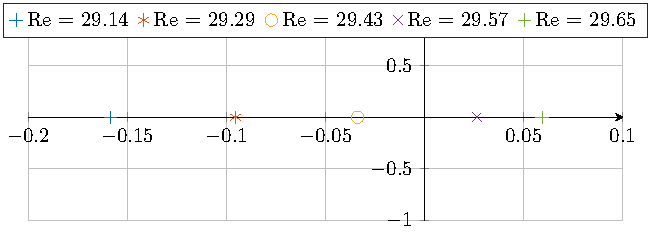
\includegraphics[width=\textwidth]{images/eigenvalues.pdf}
	\caption{Difference between values of the stream function for grid size $N\times N$ minus the value for grid size $N-32 \times N-32$}
	\label{fig:eigenvaluespitch}
\end{figure}

In this section, we will show the internal symmetry of the system (equation \ref{eq:pde}). What we will show is that if we have a steady state $\psi(x,y)$, then $-\psi(x,1-y)$ is also a steady state. The continuation start at Re=16 with an antisymmetric solution, so $\psi(x,y)=-\psi(x,1-y)$. After the pitchfork bifurcation, we get another solution, which is no longer antisymmetric. Thus its antisymmetric counterpart becomes also a solution, which gives us two new solutions. From this, we conclude that this bifurcation must be a pitchfork bifurcation.
 
 We now first show that if we have a steady state $\psi(x,y)$, then $-\psi(x,1-y)$ is also a steady state.
 
Suppose we have found a steady state $\psi(x,y)$ (we dropped the index $t$, because the steady state does not depend on $t$). Then, if we rewrite the PDE \ref{eq:pde}, we get
 \begin{equation}
   \frac{\partial}{\partial t}\zeta= - \underbrace{   u \frac{\partial\zeta}{\partial x}}_{=:\ref{eq:steady} a} +\underbrace{  v \frac{\partial\zeta}{\partial y}}_{=:\ref{eq:steady}b} - \beta \underbrace{\frac{\partial \psi}{\partial x} }_{=:\ref{eq:steady}c} - \alpha\underbrace{ \frac{\partial \tau_x}{\partial y}}_{=:\ref{eq:steady} d} +\frac{1}{Re}  \underbrace{\Delta \zeta}_{=:\ref{eq:steady}e}=0\label{eq:steady}
\end{equation}
 $$\zeta=\Delta \psi $$
For this $\psi(x,y)$.

Now we want to show that 
$$\bar{\psi}(x,y)=-\psi(x,\bar{y}) \text{ with }\bar{y}=1-y$$
is also a steady state.

So we want to show that, if equation \ref{eq:steady} holds, 
 \begin{equation} \frac{\partial}{\partial t}\bar{\zeta}=- \underbrace{  \bar u \frac{\partial\bar{\zeta}}{\partial x}}_{=:\ref{eq:othersteady} a} +\underbrace{ \bar v \frac{\partial\bar{\zeta}}{\partial y}}_{=:\ref{eq:othersteady}b} -\beta \underbrace{ \frac{\partial \bar{\psi}}{\partial x} }_{=:\ref{eq:othersteady}c} -\alpha  \underbrace{\frac{\partial \bar \tau_x}{\partial y}}_{=:\ref{eq:othersteady}d} + \frac{1}{Re} \underbrace{\Delta \bar{\zeta}}_{=:\ref{eq:othersteady}e}=0 \label{eq:othersteady}
 \end{equation}
 $$\bar{\zeta}=\Delta \bar{\psi}$$ 
We will show this by showing that the parts (a, b, c, d, e) in equation \ref{eq:othersteady} are minus the same part in equation \ref{eq:steady}. Therefore we will first show that $-\bar{u}=-u$ and $\bar{v}=v$. 
 
\begin{equation}
-\bar u=\frac{\partial \bar{\psi}}{\partial y}(x,y)=-\frac{\partial \psi}{\partial \bar y}(x,\bar y)\frac{\partial \bar{y}}{\partial y}=\frac{\partial \psi}{\partial \bar y}(x,\bar y)=-u
\label{eq:ubar}
\end{equation}

\begin{equation}
\bar v=\frac{\partial \bar{\psi}}{\partial x}(x,y)=-\frac{\partial \psi}{\partial x}(x,\bar y)=-v \label{eq:vbar}
\end{equation}

Before the further computations we will show that $\bar{\zeta}=-\zeta$.

\begin{align}
\bar{\zeta}(x,y) &= \Delta \bar{\psi}(x,y)
=\frac{\partial^2\bar{\psi}}{\partial x^2}(x, y)+\frac{\partial^2\bar{\psi}}{\partial \bar y^2}(x, y) \nonumber \\
&=-\frac{\partial^2\psi}{\partial x^2}(x,\bar y)-\frac{\partial^2\psi}{\partial \bar y^2}(x,\bar y)
=-\zeta(x,\bar y)\label{eq:zetabar}
\end{align}

With these, we will now show that equation \ref{eq:othersteady} follows from equation \ref{eq:steady}.
We start with part a of the equations. Using equations \ref{eq:ubar} and \ref{eq:zetabar},
\begin{equation*}
\ref{eq:othersteady} a=\bar u\frac{\partial\bar{\zeta}}{\partial x} (x,y) =-u \frac{\partial\zeta}{\partial x} (x,\bar y)=-\ref{eq:steady}a
\end{equation*}
Then part b, using equations \ref{eq:vbar} and \ref{eq:zetabar},
\begin{equation*}
\ref{eq:othersteady}b=\bar{v}\frac{\partial\bar{\zeta}}{\partial y} (x,y) =-v \frac{\partial\zeta}{\partial \bar y} (x,\bar y)=-\ref{eq:steady}b
\end{equation*}
Equality of the parts c follows immediately from equation \ref{eq:vbar}
$$\ref{eq:othersteady}c=\frac{\partial \bar{\psi}}{\partial x}=\bar{v}=-v=-\frac{\partial \psi}{\partial x}=-\ref{eq:steady}c$$
For part d, we have defined $\bar{\tau}_x(y)=\tau_x(\bar y)$, where we have dropped the indices $t$ and $x$, because $\tau$ does not depend on them. So we get
$$\ref{eq:othersteady}d=\frac{\partial \bar \tau_x}{\partial y}(y)=\frac{\partial \tau_x}{\partial \bar y}(\bar y)\frac{\partial y}{\partial \bar y}=-\frac{\partial \tau_x}{\partial \bar y}(\bar y)=-\ref{eq:steady}d$$
Finally we look at part e of the equations. Using equation \ref{eq:zetabar}, we get
\begin{align*}
\ref{eq:othersteady}e& =\Delta \bar{\zeta}(x,y)
=\frac{\partial^2\bar{\zeta}}{\partial x^2}(x, y)+\frac{\partial^2\bar{\zeta}}{\partial \bar y^2}(x, y) \\
&=-\frac{\partial^2\zeta}{\partial x^2}(x,\bar y)-\frac{\partial^2\zeta}{\partial \bar y^2}(x,\bar y)=-\Delta\zeta(x,\bar y)=-\ref{eq:steady} e
\end{align*}

Combining this five parts of equations \ref{eq:othersteady} and \ref{eq:steady} shows us that
$$\frac{\partial}{\partial t}\bar{\zeta}=-\frac{\partial}{\partial t}\zeta=0$$ and thus is $\bar{\psi}$ a steady state, which gives us the internal symmetry of the system that gives rise to the pitchfork bifurcation.



